% !TeX root = ../main.tex
%% =======================================================================
%  CAPITULO 8 — VALIDACION EXPERIMENTAL
\chapter{Validaci\'on experimental}
\label{cap:experimental}

\section{Introducci\'on}
\label{sec:exp-intro}

En este cap\'itulo se implementa la cadena \'optica en el laboratorio y se
procesan las se\~nales adquiridas utilizando la misma cadena DSP desarrollada
y evaluada mediante simulaciones en los cap\'itulos anteriores.

El objetivo es validar experimentalmente el procesamiento digital, no
reproducir el enlace satelital completo. El sistema implementado consiste en
un enlace de fibra \'optica entre un transmisor y un receptor coherente, por
lo que no contempla efectos como la p\'erdida de espacio libre, la
amplificaci\'on \'optica de potencia o la rotaci\'on din\'amica del estado de
polarizaci\'on. Sin embargo, permite evaluar el desempe\~no del DSP frente a
imperfecciones reales de los dispositivos, que en las simulaciones se
representan mediante modelos aproximados. Entre ellas se encuentran el ruido
de fase de los l\'aseres, los desbalances y las limitaciones de ancho de banda
del front end, el desfasaje temporal entre canales y las imperfecciones del
proceso de adquisici\'on.

La validaci\'on experimental comprende tres ensayos. El primero eval\'ua el
desempe\~no del receptor para tres tasas de s\'imbolo, \SI{12.5}{\giga\baud},
\SI{25}{\giga\baud} y \SI{32}{\giga\baud}, correspondientes a tasas de
transmisi\'on de \SI{50}{\giga\bit\per\second},
\SI{100}{\giga\bit\per\second} y \SI{128}{\giga\bit\per\second}. El segundo
caracteriza la sensibilidad del receptor mediante la variaci\'on de la
potencia \'optica de la se\~nal recibida y del oscilador local, con el
objetivo de determinar las condiciones m\'inimas de potencia necesarias para
su funcionamiento. Finalmente, el tercero reproduce el desplazamiento de
frecuencia asociado al efecto Doppler mediante el ajuste de la frecuencia
\'optica del transmisor, para evaluar el rango de offsets que el receptor
puede compensar.


\section{Esquema experimental}
\label{sec:exp-banco}

\begin{figure}[H]
  \centering
  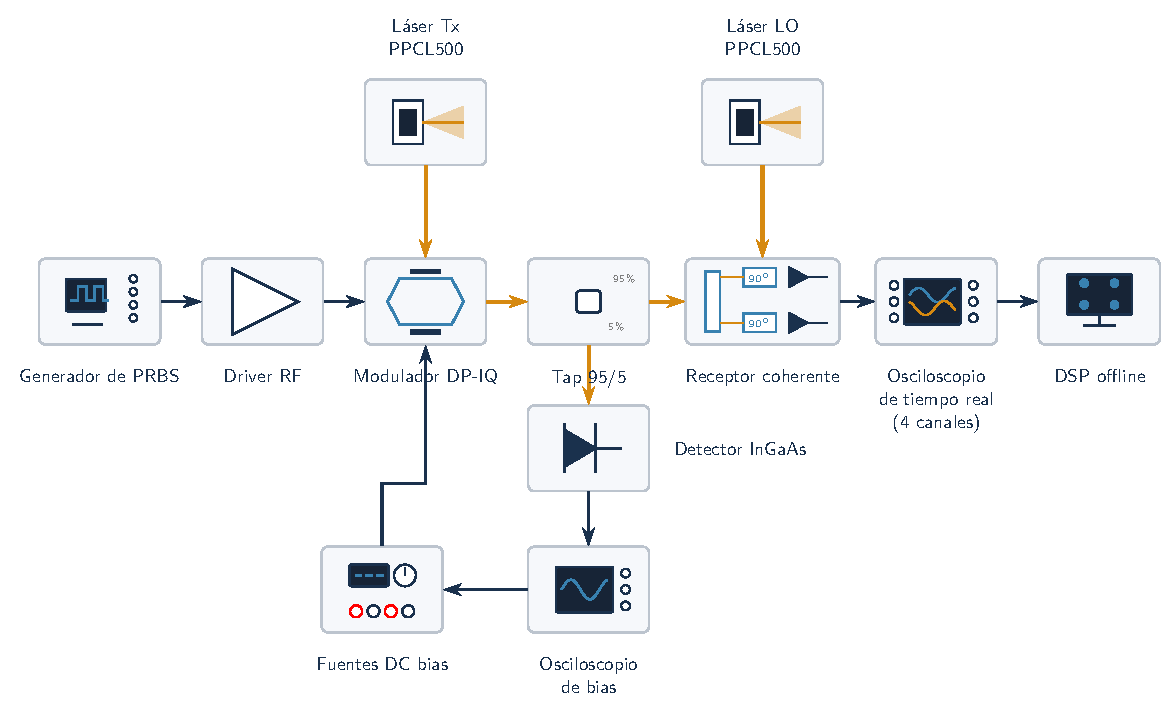
\includegraphics[width=\textwidth]{figuras/lab_setup_base.pdf}
  \caption[Esquema de medici\'on coherente DP-QPSK]{%
    Esquema de la configuraci\'on experimental. Los caminos \'opticos y
    el\'ectricos se indican en naranja y azul, respectivamente. La salida del
    \SI{5}{\percent} del acoplador \'optico se utiliza para alimentar el lazo
    de control del punto de polarizaci\'on (\emph{bias}) del modulador.}
  \label{fig:exp-setup}
\end{figure}

La \cref{fig:exp-setup} muestra el esquema completo de la configuraci\'on
experimental.

El generador de patrones produce cuatro secuencias PRBS independientes, una
para cada rama del modulador, correspondientes a las componentes en fase y
cuadratura de ambas polarizaciones. Un driver de RF de cuatro canales
amplifica estas se\~nales para alcanzar la excursi\'on de tensi\'on requerida
por el modulador. Como se explic\'o en la \cref{sec:trx-modulador}, cada
modulador Mach-Zehnder se polariza en el punto de m\'inima transmisi\'on. 

La portadora \'optica es generada por el l\'aser transmisor, un ITLA
sintonizable en la banda C, la cual ingresa al modulador de doble
polarizaci\'on. Dado que los puntos de operaci\'on de los moduladores no
permanecen constantes en el tiempo, sino que presentan derivas debido
principalmente a variaciones de temperatura y otras condiciones ambientales,
las seis tensiones de polarizaci\'on deben ajustarse din\'amicamente para
mantener las condiciones de operaci\'on deseadas. Para ello se dispone de un
lazo de control autom\'atico de bias. En concreto, a la salida del modulador
se dispone un tramo corto de fibra monomodo y un acoplador \'optico que divide
la potencia en dos ramas, del \SI{95}{\percent} y el \SI{5}{\percent}. La
primera se dirige hacia el receptor coherente, mientras que la segunda
alimenta un fotodetector de InGaAs. La se\~nal resultante es adquirida por un
osciloscopio y se utiliza como realimentaci\'on del algoritmo de control, que
ajusta las fuentes de tensi\'on continua para mantener los puntos de
operaci\'on del modulador.

Se utiliza otro l\'aser ITLA del mismo modelo que el transmisor como LO, que
se conecta directamente al receptor, es decir, el front-end \'optico. Dentro
se encuentra el par de h\'ibridos de \SI{90}{\degree} que baten la se\~nal contra el
oscilador local, y los cuatro pares de fotodiodos balanceados con sus
amplificadores de transimpedancia. El receptor genera as\'i cuatro tensiones,
que contienen la fase y cuadratura de cada polarizaci\'on.

El osciloscopio digitaliza estos cuatro canales. Por \'ultimo, las capturas se
guardan y se procesan despu\'es en MATLAB con la misma cadena de bloques del
cap\'itulo~\ref{cap:dsp}.

\begin{table}[htbp]
  \centering

  \begin{tabular}{lll}
    \toprule
    Funci\'on & Equipo & Caracter\'istica relevante \\
    \midrule
    Generador de patrones & Tektronix PPG3204      & cuatro canales, PRBS \\
    L\'aser Tx y LO       & Pure Photonics PPCL500 & sinton\'ia fina de $\pm\SI{30}{\giga\hertz}$ \\
    Front end coherente   & Lab Buddy DSC-R413     & h\'ibrido de \SI{90}{\degree} y balanceados \\
    Digitalizador         & Tektronix DPO70000SX   & \SI{50}{\giga S\per\second} por canal \\
    Control de bias       & Tektronix MDO3054      & lectura del detector del tap \\
    \bottomrule
  \end{tabular}
  \caption[Equipos utilizados en el laboratorio]{%
    Equipos utilizados y la caracter\'istica que importa en cada caso.}
  \label{tab:instrumental}
\end{table}


\section{Desempe\~no en t\'erminos de BER y EVM}
\label{sec:exp-tasas}
\label{sec:exp-osnr}

Se realizaron mediciones correspondientes a las tres tasas de transmisi\'on
consideradas, cambiando \'unicamente la frecuencia de reloj del generador y la
frecuencia de muestreo del osciloscopio. Las
\cref{fig:exp-const-125,fig:exp-const-25,fig:exp-const-32} muestran las
constelaciones recuperadas.

\begin{figure}[H]
  \centering
  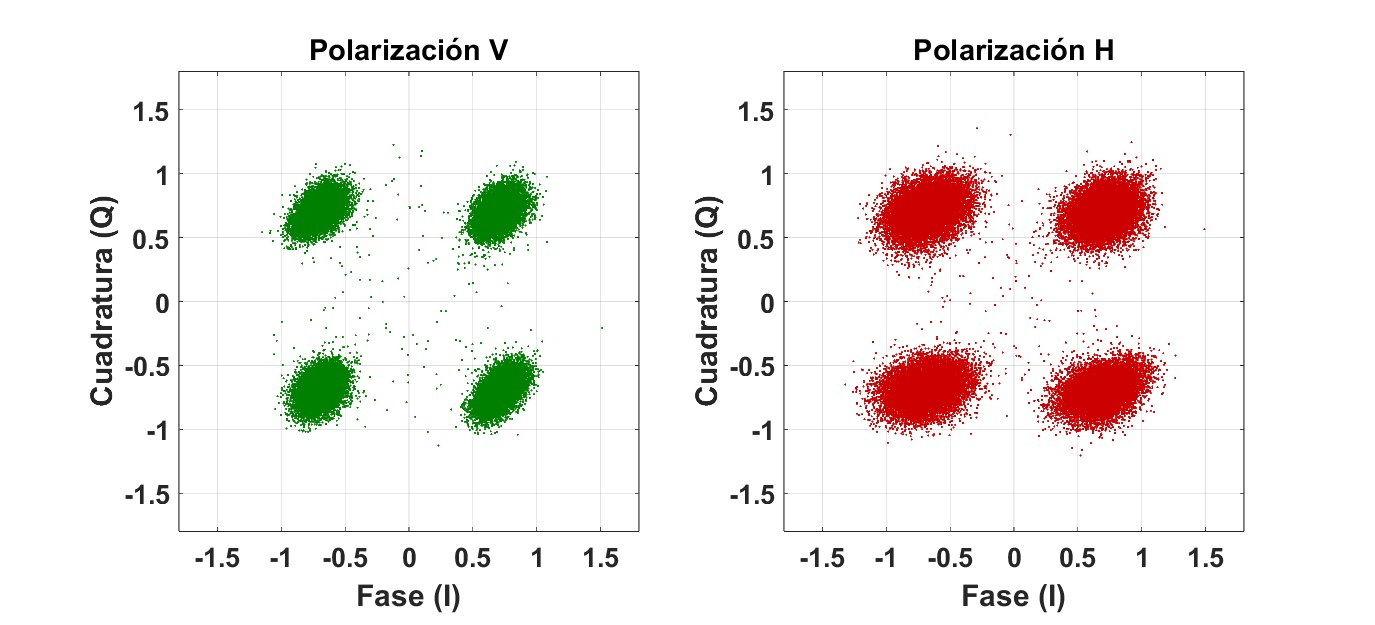
\includegraphics[width=0.95\textwidth]{figuras/Lab_12p5Gb_Final.jpg}
  \caption[Constelaci\'on medida a \SI{12.5}{\giga\baud}]{%
    Constelaci\'on recuperada de una captura de laboratorio a
    \SI{12.5}{\giga\baud}, equivalente a \SI{50}{\giga\bit\per\second}, con un
    EVM de \SI{16}{\percent}.}
  \label{fig:exp-const-125}
\end{figure}

\begin{figure}[H]
  \centering
  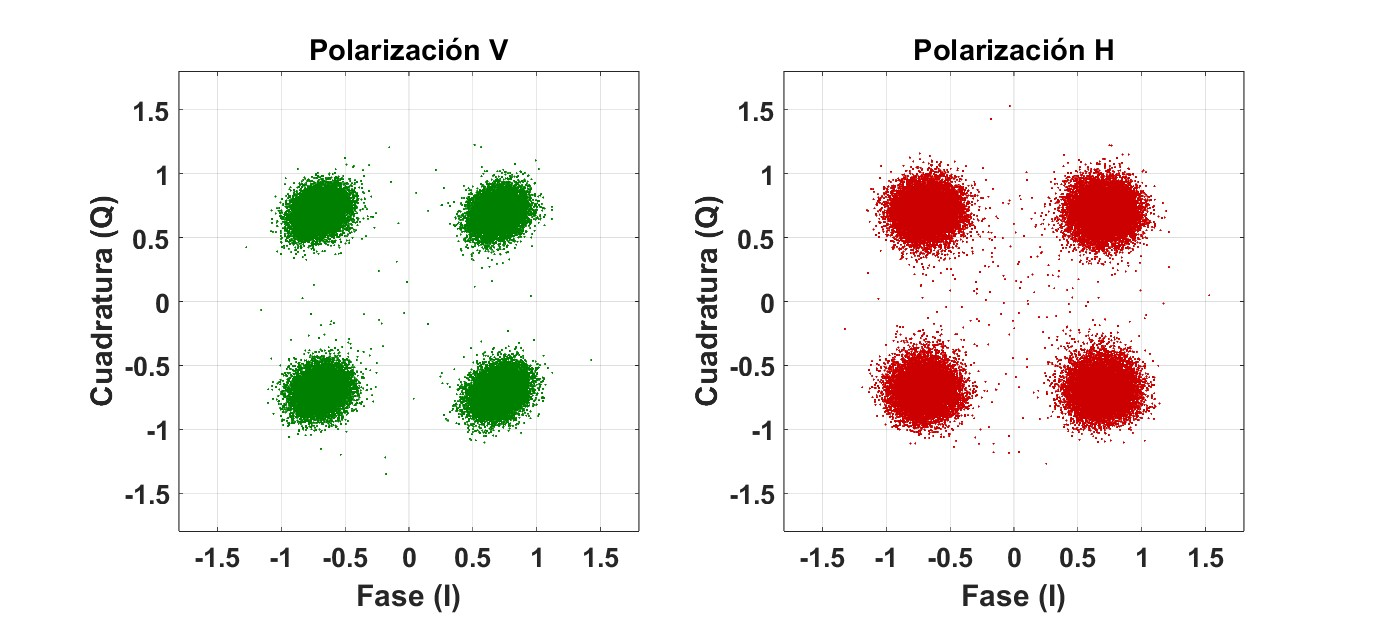
\includegraphics[width=0.95\textwidth]{figuras/Lab_25Gb_Final.jpg}
  \caption[Constelaci\'on medida a \SI{25}{\giga\baud}]{%
    Constelaci\'on recuperada a \SI{25}{\giga\baud}, equivalente a
    \SI{100}{\giga\bit\per\second}, con un EVM de \SI{22}{\percent}.}
  \label{fig:exp-const-25}
\end{figure}

\begin{figure}[H]
  \centering
  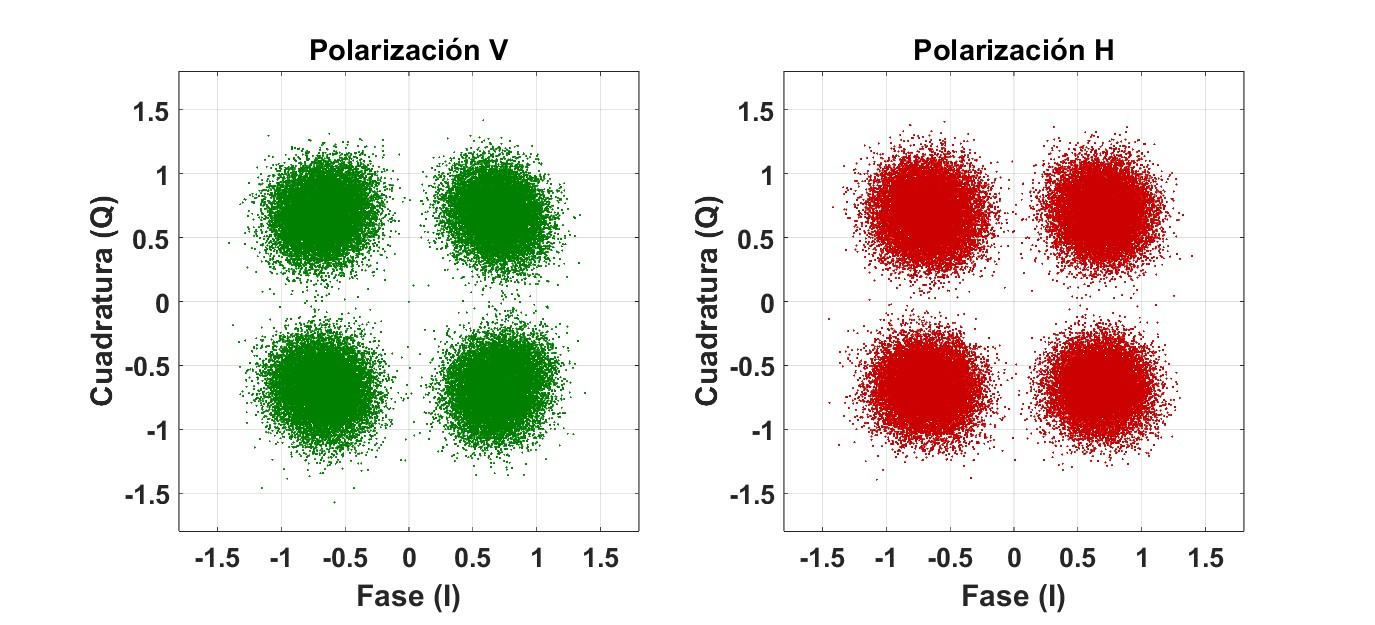
\includegraphics[width=0.95\textwidth]{figuras/Lab_32Gb_Final.jpg}
  \caption[Constelaci\'on medida a \SI{32}{\giga\baud}]{%
    Constelaci\'on recuperada a \SI{32}{\giga\baud}, equivalente a
    \SI{128}{\giga\bit\per\second}, que es la tasa de dise\~no del enlace, con
    un EVM de \SI{33}{\percent}.}
  \label{fig:exp-const-32}
\end{figure}

Se observan en los tres casos las constelaciones de QPSK y las dos
polarizaciones separadas. Por lo tanto, la cadena de procesamiento
demultiplexa, recupera el reloj, corrige el offset de frecuencia y engancha la
fase sobre se\~nales reales. Sin embargo, se observa que las nubes de
s\'imbolos no tienen la simetr\'ia circular propia de un canal AWGN. Esto
sugiere que hay cierto desbalance de cuadratura residual presente en
los s\'imbolos finales.

La diferencia entre las tres est\'a en el tama\~no de las nubes. A
\SI{12.5}{\giga\baud} los c\'umulos son compactos y quedan bien separados de
los ejes. A \SI{25}{\giga\baud} crecen de manera apreciable. A
\SI{32}{\giga\baud} el radio de cada nube es comparable a la distancia al eje,
y algunos s\'imbolos cruzan al cuadrante vecino, generando los primeros
errores contados.

En los experimentos de laboratorio no se dispuso de una medici\'on directa de
la OSNR. Por esta raz\'on se estim\'o una OSNR equivalente a partir de las
constelaciones recuperadas por el DSP, utilizando las relaciones del
\cref{cap:coherentes}. La magnitud del vector de error se relaciona con la relaci\'on
se\~nal-ruido mediante la \eqref{eq:evm-ber}, y la \eqref{eq:osnr-esno} la
refiere al ancho de banda de referencia de \SI{12.5}{\giga\hertz}.

Esta cifra es una OSNR equivalente y no una medici\'on \'optica. El EVM
incorpora tambi\'en degradaciones distintas del ruido \'optico, como el error
residual de ecualizaci\'on, el ruido de fase y las imperfecciones del
transmisor y del receptor. Por lo tanto, el valor estimado no coincide
necesariamente con la OSNR que se medir\'ia de forma directa con un analizador
de espectro \'optico.

\begin{table}[htbp]
  \centering

  \begin{tabular}{lccccc}
    \toprule
    Tasa & $\Rs$ & $\EVM$ & $E_s/N_0$ & $\OSNR$ equivalente & BER estimada \\
    \midrule
    \SI{50}{\giga\bit\per\second}  & \SI{12.5}{\giga\baud} & \SI{16}{\percent} & \SI{15.9}{\dB} & \SI{15.9}{\dB} & \num{2e-10} \\
    \SI{100}{\giga\bit\per\second} & \SI{25}{\giga\baud}   & \SI{22}{\percent} & \SI{13.2}{\dB} & \SI{16.2}{\dB} & \num{2.7e-6} \\
    \SI{128}{\giga\bit\per\second} & \SI{32}{\giga\baud}   & \SI{33}{\percent} & \SI{9.6}{\dB}  & \SI{13.7}{\dB} & \num{1.2e-3} \\
    \bottomrule
  \end{tabular}
  \caption[OSNR equivalente estimada en el banco]{%
    EVM medido en cada tasa, con la relaci\'on se\~nal-ruido y la OSNR
    equivalente que resultan. La columna $E_s/N_0$ es la relaci\'on
    el\'ectrica en el punto de decisi\'on.}
  \label{tab:exp-osnr}
\end{table}

En la \cref{tab:exp-osnr} se muestra la OSNR equivalente estimada para las
tasas de transmisi\'on consideradas. La potencia \'optica es la misma en las
tres medidas, ya que se us\'o la misma potencia de l\'aser, y la densidad
espectral de ruido tambi\'en, as\'i que al duplicar la tasa de s\'imbolo se
integra el doble de ruido y la relaci\'on cae \SI{3}{\dB}. Entre
\SI{12.5}{\giga\baud} y \SI{25}{\giga\baud} la ca\'ida medida es de
\SI{2.8}{\dB} contra \SI{3.0}{\dB} que predice la cuenta. Por lo tanto, la
transici\'on de \SI{50}{\giga\bit\per\second} a
\SI{100}{\giga\bit\per\second}, a estas potencias en el receptor, no degrada
nada que no sea directamente la penalidad por ancho de banda. En el tercer
experimento se analiza en mayor detalle. La OSNR equivalente, que no tiene en
cuenta este factor, queda pr\'acticamente igual en las dos tasas.

Por otro lado, el pasar de \SI{25}{\giga\baud} a \SI{32}{\giga\baud}
deber\'ia implicar \SI{1.1}{\dB} de relaci\'on se\~nal-ruido por ancho de banda y, sin embargo, se obtiene una diferencia de \SI{3.5}{\dB}. Hay por lo tanto \SI{2.4}{\dB} de exceso, y la OSNR equivalente cae de \SI{16.2}{\dB} a
\SI{13.7}{\dB}. Este exceso tiene tres contribuciones debidas al equipo
utilizado.

\paragraph{L\'imite de tasa de muestreo del osciloscopio}
El osciloscopio puede muestrear como m\'aximo a \SI{50}{\giga S\per\second}
por canal. A \SI{12.5}{\giga\baud} y \SI{25}{\giga\baud} esto alcanza para
capturar a dos muestras por s\'imbolo, que es la tasa a la que trabaja el DSP.
A \SI{32}{\giga\baud} se obtienen \num{1.5625} muestras por s\'imbolo y el DSP
tiene que interpolar hasta \num{2} antes de empezar. La
\cref{tab:sps-captura} resume la situaci\'on.

La interpolaci\'on aumenta la cantidad de muestras pero no agrega
informaci\'on. Con \SI{50}{\giga S\per\second} el l\'imite de Nyquist de la
captura queda en \SI{25}{\giga\hertz}, por debajo del contenido espectral que
la se\~nal NRZ a \SI{32}{\giga\baud} tiene por encima de esa frecuencia, de
modo que parte del espectro se pliega ya en la adquisici\'on. Lo que se pierde
en ese plegado no se recupera despu\'es en el procesamiento.

\begin{table}[htbp]
  \centering

  \begin{tabular}{lccc}
    \toprule
    Tasa & $\Rs$ & $F_s$ del osciloscopio & Muestras por s\'imbolo \\
    \midrule
    \SI{50}{\giga\bit\per\second}  & \SI{12.5}{\giga\baud} & \SI{25}{\giga S\per\second} & 2 \\
    \SI{100}{\giga\bit\per\second} & \SI{25}{\giga\baud}   & \SI{50}{\giga S\per\second} & 2 \\
    \SI{128}{\giga\bit\per\second} & \SI{32}{\giga\baud}   & \SI{50}{\giga S\per\second} & \num{1.5625} \\
    \bottomrule
  \end{tabular}
  \caption[Muestras por s\'imbolo en la captura]{%
    Frecuencia de muestreo y muestras por s\'imbolo disponibles en cada tasa.
    S\'olo la tasa de dise\~no queda por debajo de las dos muestras por
    s\'imbolo que necesita el DSP.}
  \label{tab:sps-captura}
\end{table}

\paragraph{El ancho de banda del camino el\'ectrico}
Los amplificadores de transimpedancia del front end y los drivers de
radiofrecuencia presentan una respuesta en frecuencia no plana, con una
atenuaci\'on creciente hacia las frecuencias m\'as altas del espectro de la
se\~nal. Esta limitaci\'on introduce distorsi\'on en la forma de los pulsos y
genera interferencia entre s\'imbolos, mucho m\'as nociva a
\SI{32}{\giga\baud} que a \SI{25}{\giga\baud} y \SI{12.5}{\giga\baud}. Si bien
el ecualizador adaptativo puede compensar parcialmente esta distorsi\'on, su
capacidad est\'a limitada por la amplificaci\'on del ruido que se produce al
intentar invertir la atenuaci\'on de las componentes espectrales de alta
frecuencia.

\paragraph{El skew entre ramas}
El cap\'itulo~\ref{cap:tolerancias} mostr\'o que el skew entre las ramas en
fase y cuadratura es el deterioro de margen m\'as estrecho de todo el
receptor, y que su efecto crece con la frecuencia. Ese retardo no proviene
\'unicamente del front end de recepci\'on, ya que el transmisor tambi\'en
introduce diferencias de camino entre las cuatro ramas. La tasa de
\SI{32}{\giga\baud} es la de mayor ancho de banda de las tres analizadas, de
modo que el mismo retardo f\'isico degrada m\'as la se\~nal.

Como conclusi\'on, se procesaron muestras a la tasa de dise\~no, con una OSNR
equivalente de \SI{13.7}{\dB}, un dec\'ibel por encima del umbral HD-FEC. Se
pudo recuperar la constelaci\'on QPSK en ambas polarizaciones.


\section{Barridos de potencia}
\label{sec:exp-barridos}

Las mediciones anteriores se realizaron para una \'unica condici\'on de
potencia \'optica recibida. En esta secci\'on se caracteriza el desempe\~no
del receptor en funci\'on de la potencia \'optica, con el objetivo de
determinar los niveles m\'inimos necesarios para su funcionamiento. Para ello
se realizaron dos barridos independientes, uno variando la potencia de la
se\~nal recibida y otro modificando la potencia del oscilador local.

Para realizar estas mediciones se introdujeron dos modificaciones en el
esquema experimental de la \cref{fig:exp-setup}. En primer lugar, se
reemplaz\'o el l\'aser transmisor por un ID Photonics CoBrite Tunable Laser
DX, que proporciona una mayor potencia \'optica de salida y permite ampliar el
rango de potencias evaluado. En segundo lugar, se incorpor\'o un atenuador
\'optico variable entre el acoplador 95/5 y el receptor coherente, para
controlar la potencia de se\~nal incidente sin modificar las condiciones de
operaci\'on del modulador. El esquema experimental resultante se presenta en
la \cref{fig:exp-setup-barrido}.

\begin{figure}[H]
  \centering
  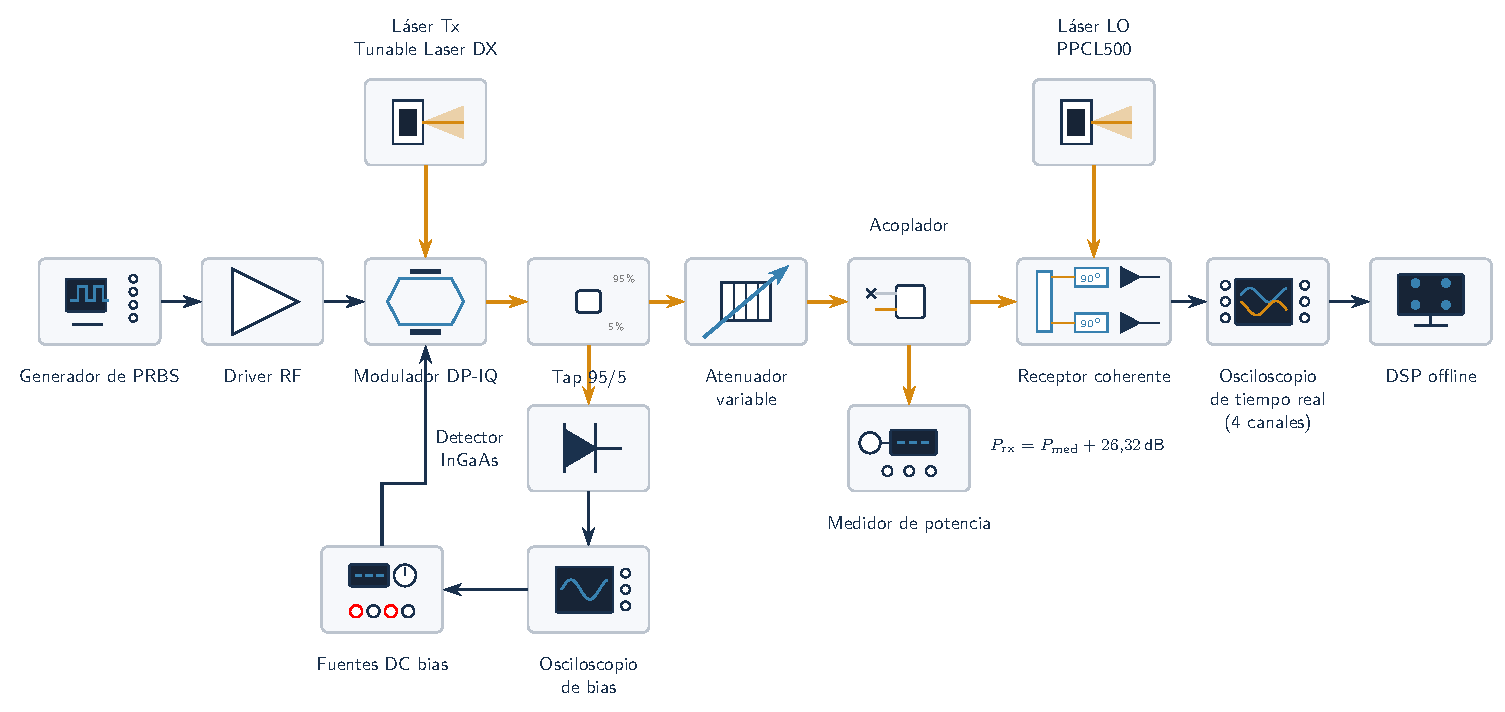
\includegraphics[width=\textwidth]{figuras/lab_setup_barrido.pdf}
  \caption[Esquema de medici\'on con atenuador variable]{%
    Esquema experimental utilizado para los barridos de potencia \'optica.
    Respecto de la configuraci\'on de la \cref{fig:exp-setup}, se incorpora un
    atenuador \'optico variable y un sistema de monitoreo compuesto por un
    acoplador \'optico y un medidor de potencia, que permite estimar la
    potencia \'optica incidente sobre el receptor.}
  \label{fig:exp-setup-barrido}
\end{figure}


Para estimar la potencia \'optica incidente sobre el receptor se incorpor\'o
un acoplador de fibra sintonizable, a modo de tap, ubicado despu\'es del
atenuador variable. Una de sus salidas se conecta al front end del receptor
coherente y la otra a un medidor de potencia \'optica. Se utiliz\'o una
relaci\'on de acoplamiento que permite dirigir la mayor parte de la potencia
hacia el receptor, manteniendo en la rama de monitoreo un nivel de potencia
suficiente para realizar una medici\'on confiable.

La diferencia de potencia entre ambas ramas se determin\'o mediante una
calibraci\'on experimental, obteni\'endose un valor de
$\Delta_{\mathrm{cal}} = \SI{26.3}{\dB}$. De esta manera, la potencia
\'optica incidente sobre el receptor puede calcularse a partir de la lectura
del medidor como
\begin{equation}
  P_{\mathrm{rx}} = P_{\mathrm{medidor}} + \Delta_{\mathrm{cal}},
  \label{eq:exp-calibracion}
\end{equation}
donde ambas potencias se expresan en \si{\dBm}. La calibraci\'on se
repiti\'o al inicio de cada sesi\'on de medici\'on y despu\'es de realizar
modificaciones en la cadena \'optica.

\subsection{Barrido de potencia de la se\~nal recibida}
\label{sec:exp-barrido-tx}

Manteniendo fija la potencia del oscilador local en su punto de trabajo
(\SI{8.0}{\dBm}), se reduce progresivamente la potencia \'optica de la
se\~nal recibida mediante el atenuador variable, en pasos de aproximadamente
\SI{0.5}{\dB}. En cada punto del barrido se realizan ocho capturas del
osciloscopio, que posteriormente se procesan con la cadena DSP del receptor.

Para cada nivel de potencia se obtienen dos estimaciones de la tasa de error
de bits. La primera se calcula por conteo directo, comparando la secuencia de
bits recuperada con la PRBS transmitida y acumulando los errores de las ocho
capturas. Dado que este m\'etodo tiene una resoluci\'on limitada por la
cantidad total de bits analizados, solo se representan los puntos con una
cantidad suficiente de errores para obtener una estimaci\'on confiable. La
segunda se obtiene a partir del EVM de la constelaci\'on recuperada,
siguiendo el procedimiento descrito en la \cref{sec:exp-osnr}. Ambos
resultados se presentan por separado para cada polarizaci\'on.

\begin{figure}[H]
  \centering
  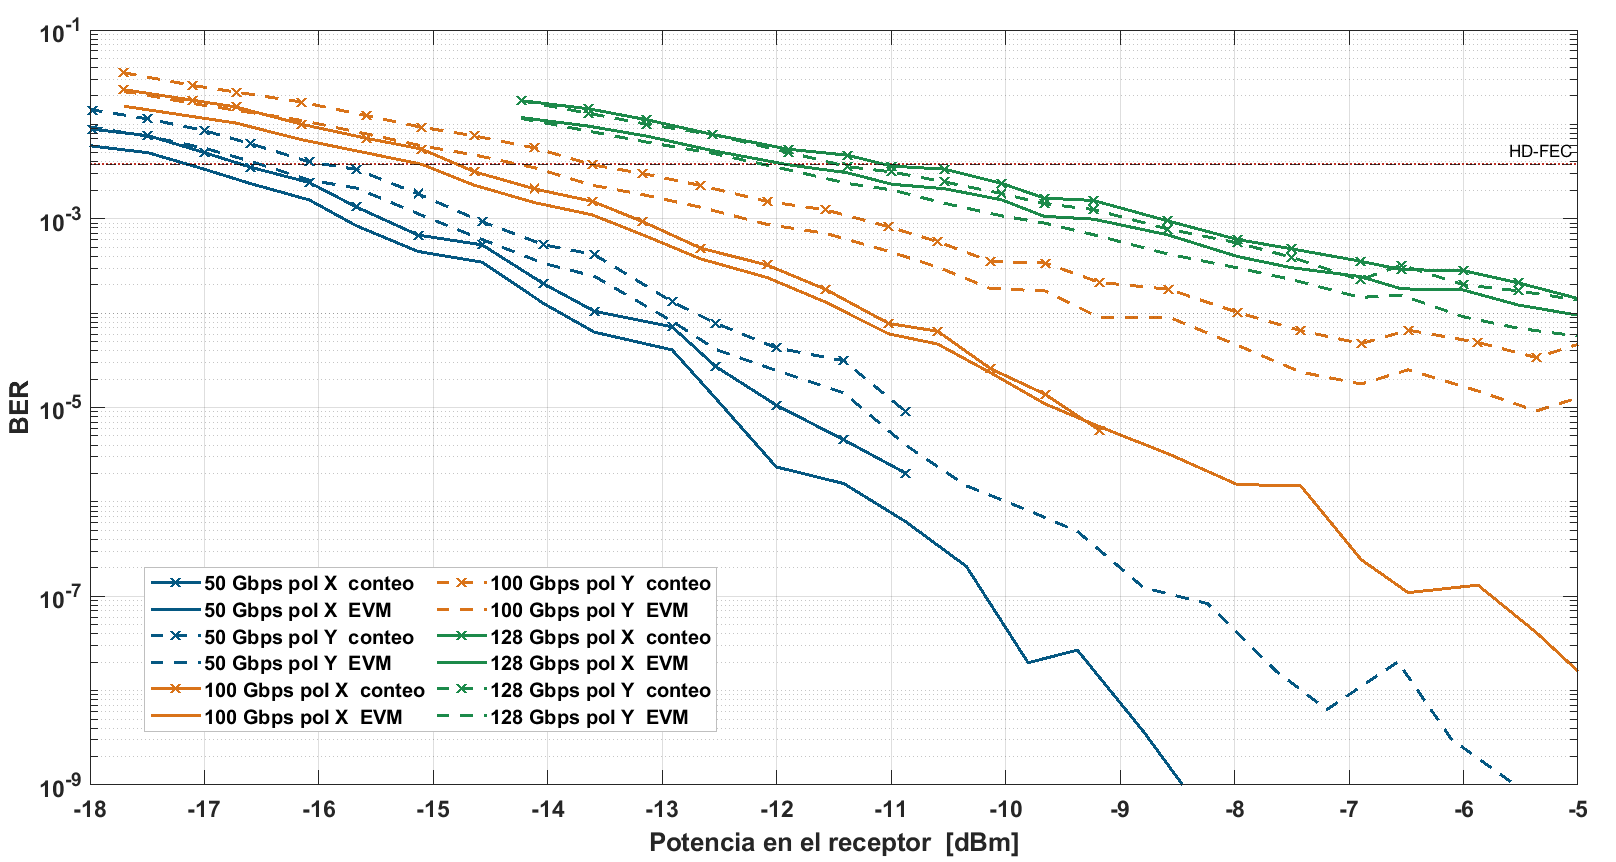
\includegraphics[width=\textwidth]{figuras/BarridoTxTodasLasTasas.png}
  \caption[Barrido de potencia de se\~nal en las tres tasas]{%
    BER en funci\'on de la potencia \'optica en el receptor para las tres
    tasas. El color indica la tasa, la l\'inea llena y la de trazos las
    polarizaciones X e Y, y las cruces la BER contada contra la estimada por
    EVM. La l\'inea punteada es el umbral HD-FEC.}
  \label{fig:exp-barrido-tx}
\end{figure}

La \cref{fig:exp-barrido-tx} muestra los resultados obtenidos para las tres
tasas de s\'imbolo, en un rango de potencia \'optica recibida de
\SIrange{-18}{-5}{\dBm}. Como era de esperar, el desempe\~no del receptor
mejora al aumentar la potencia de se\~nal. Tambi\'en se observa que una de las
polarizaciones presenta una BER sistem\'aticamente mayor en todo el rango
medido, lo que sugiere la existencia de diferencias en las caracter\'isticas
de los caminos de transmisi\'on o recepci\'on de ambas polarizaciones.

Tomando como referencia el cruce con el umbral HD-FEC de la BER medida por
conteo en la polarizaci\'on de peor desempe\~no, se obtiene una sensibilidad
de \SI{-16.0}{\dBm} a \SI{12.5}{\giga\baud}, \SI{-13.6}{\dBm} a
\SI{25}{\giga\baud} y \SI{-11.0}{\dBm} a \SI{32}{\giga\baud}. La diferencia
entre los dos primeros valores, de \SI{2.4}{\dB}, es cercana al incremento
te\'orico de \SI{3}{\dB} en la potencia requerida al duplicar la tasa de
s\'imbolo, manteniendo constante la relaci\'on se\~nal-ruido por s\'imbolo.
En cambio, el incremento de \SI{2.6}{\dB} observado al pasar de
\SI{25}{\giga\baud} a \SI{32}{\giga\baud} supera los \SI{1.1}{\dB} esperados
por el cambio de tasa. Esta diferencia es consistente con la penalidad
adicional observada a la tasa de dise\~no en la \cref{sec:exp-osnr}, que
ac\'a se manifiesta como un aumento de la potencia necesaria para alcanzar el
umbral de BER.

Por \'ultimo, la BER estimada a partir del EVM presenta una tendencia similar
a la BER medida por conteo, lo que respalda su utilidad como m\'etodo de
estimaci\'on indirecta.

La \cref{tab:exp-cruces-tx} resume las sensibilidades obtenidas para cada tasa
de s\'imbolo y polarizaci\'on.

% ---------------------------------------------------------------
\begin{table}[htbp]
  \centering

  \begin{tabular}{lccc}
    \toprule
    Tasa & Pol.\ X & Pol.\ Y & Diferencia \\
    \midrule
    \SI{50}{\giga\bit\per\second} & \SI{-16.68}{\dBm} & \SI{-15.97}{\dBm} & \SI{0.72}{\dB} \\
    \SI{100}{\giga\bit\per\second} & \SI{-14.80}{\dBm} & \SI{-13.63}{\dBm} & \SI{1.17}{\dB} \\
    \SI{128}{\giga\bit\per\second} & \SI{-11.52}{\dBm} & \SI{-11.03}{\dBm} & \SI{0.49}{\dB} \\
    \bottomrule
  \end{tabular}
  \caption[Cruce del umbral HD-FEC en el barrido de se\~nal]{%
    Potencia \'optica de se\~nal en el receptor a la que la BER contada de
    cada polarizaci\'on cruza el umbral HD-FEC, y diferencia entre las dos.}
  \label{tab:exp-cruces-tx}
\end{table}

\subsection{Barrido de potencia del oscilador local}
\label{sec:exp-barrido-lo}

En el segundo barrido se mantuvo fija la potencia \'optica de la se\~nal
recibida en \SI{-5.5}{\dBm} y se vari\'o la potencia del LO. Dado que el
l\'aser permite ajustar directamente su potencia de salida entre
\SIrange{7}{13}{\dBm}, las mediciones se realizaron en dos etapas. En la
primera, el LO se conect\'o directamente al receptor para cubrir el rango de
potencias m\'as altas. En la segunda, se incorpor\'o un atenuador fijo de
\SI{7.7}{\dB} a la salida del l\'aser para extender las mediciones hacia
potencias menores. De esta manera se cubri\'o un rango de
\SIrange{-0.3}{11}{\dBm} de potencia \'optica del LO incidente sobre el front
end. El procesamiento de las se\~nales y el c\'alculo de la BER se realizaron
siguiendo el mismo procedimiento que en el barrido anterior.

\begin{figure}[H]
  \centering
  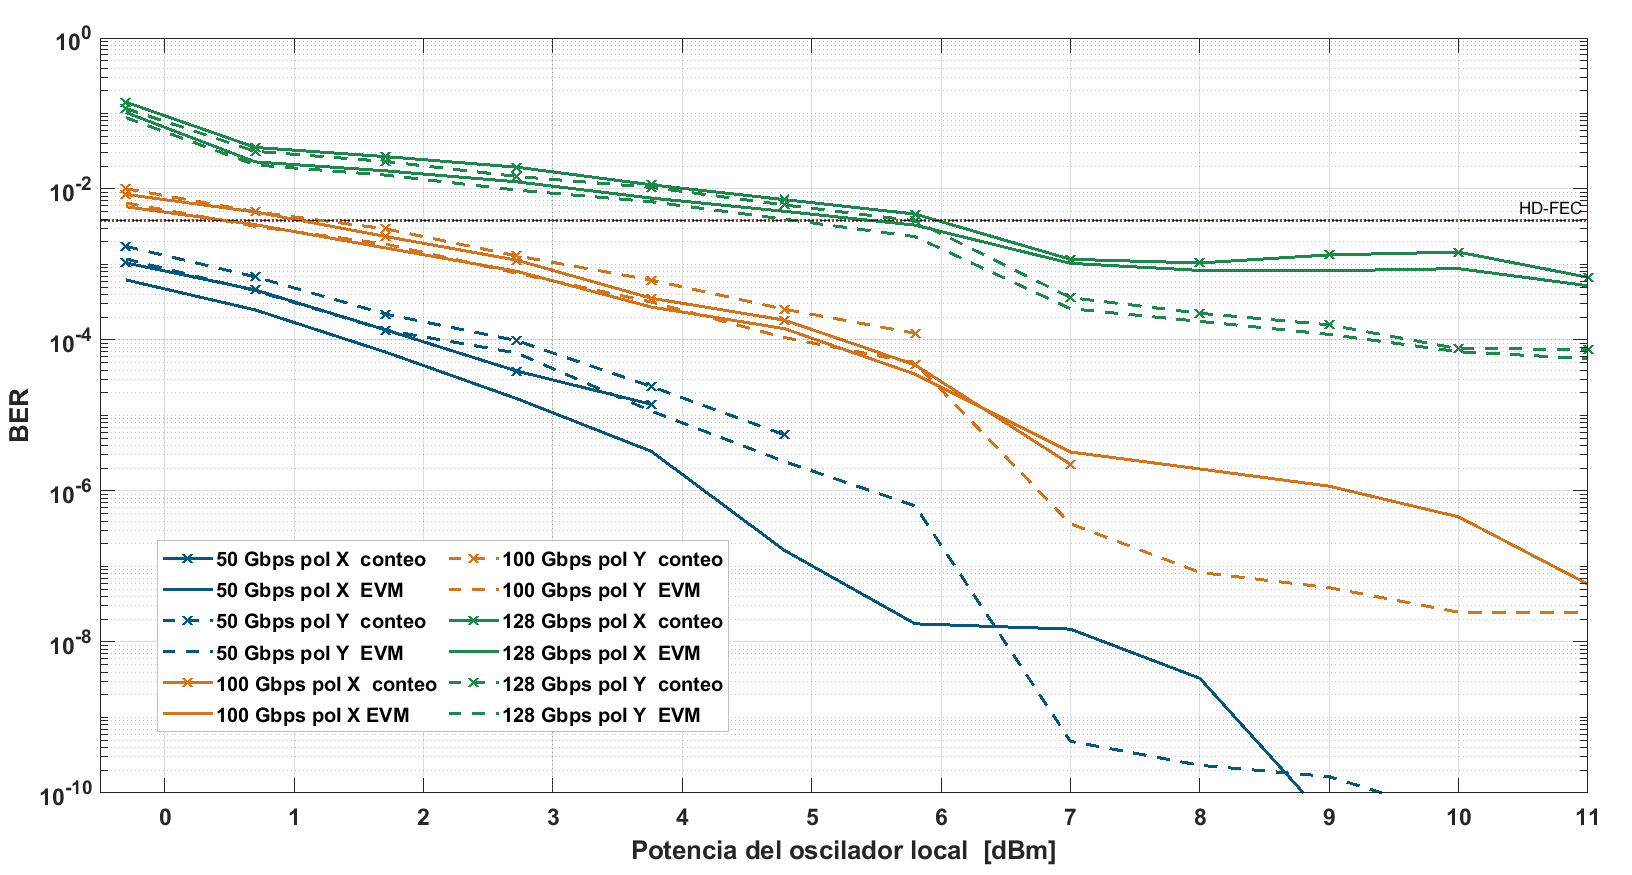
\includegraphics[width=\textwidth]{figuras/BarridoLOTodasLasTasas.png}
  \caption[Barrido de potencia de oscilador local en las tres tasas]{%
    BER en funci\'on de la potencia de oscilador local en el receptor para las
    tres tasas, con la potencia de se\~nal fija en \SI{-5.5}{\dBm}. La
    convenci\'on de colores, l\'ineas y marcadores es la misma que la de la
    \cref{fig:exp-barrido-tx}.}
  \label{fig:exp-barrido-lo}
\end{figure}

La \cref{fig:exp-barrido-lo} muestra los resultados obtenidos. Las curvas
presentan un comportamiento similar para las tres tasas de transmisi\'on. A
bajas potencias del LO, la BER disminuye r\'apidamente al aumentar su
potencia. A partir de aproximadamente \SI{7}{\dBm} la mejora se vuelve
considerablemente menor y, para \SI{128}{\giga\bit\per\second}, la BER
permanece pr\'acticamente constante entre \SI{7}{\dBm} y \SI{11}{\dBm}.

Este comportamiento es consistente con el esperado para un receptor coherente.
La amplitud de la corriente de batido es proporcional a la ra\'iz del producto
de las potencias \'opticas de la se\~nal y del oscilador local. Por lo tanto,
manteniendo fija la potencia de se\~nal, la potencia el\'ectrica de la se\~nal
detectada crece proporcionalmente con la potencia del LO. Mientras predomina
el ruido t\'ermico de la electr\'onica de recepci\'on, cuya potencia es
aproximadamente independiente del LO, cada incremento de \SI{1}{\dB} en su
potencia produce una mejora cercana a \SI{1}{\dB} en la relaci\'on
se\~nal-ruido el\'ectrica. Sin embargo, al aumentar la potencia del oscilador
local tambi\'en crece el ruido de disparo asociado a la fotocorriente, cuya
varianza es proporcional a la potencia \'optica recibida. Cuando este ruido
predomina, tanto la potencia el\'ectrica de se\~nal como la potencia de ruido
aumentan aproximadamente en la misma proporci\'on, por lo que la relaci\'on
se\~nal-ruido deja de mejorar de forma significativa.

El aplanamiento observado en las curvas indica que, a partir de cierta
potencia del LO, su incremento deja de producir una mejora apreciable en el
desempe\~no. En este r\'egimen la BER queda limitada por las restantes
contribuciones de ruido y distorsi\'on del sistema, incluyendo las
degradaciones identificadas en la \cref{sec:exp-osnr}.

A \SI{50}{\giga\bit\per\second} la BER permanece por debajo del umbral HD-FEC
en todo el rango medido. Para \SI{100}{\giga\bit\per\second} y
\SI{128}{\giga\bit\per\second}, los cruces con este umbral se producen a
potencias del LO de \SI{1.23}{\dBm} y \SI{5.98}{\dBm}, respectivamente,
tomando como referencia la BER medida por conteo en la polarizaci\'on de peor
desempe\~no.

La \cref{tab:exp-cruces-lo} resume las potencias m\'inimas del oscilador local
necesarias para alcanzar el umbral HD-FEC en cada tasa de transmisi\'on y
polarizaci\'on.

% ---------------------------------------------------------------
\begin{table}[htbp]
  \centering

  \begin{tabular}{lccc}
    \toprule
    Tasa & Pol.\ X & Pol.\ Y & Diferencia \\
    \midrule
    \SI{50}{\giga\bit\per\second}$^{*}$ & \SI{-1.45}{\dBm} & \SI{-1.04}{\dBm} & \SI{0.41}{\dB} \\
    \SI{100}{\giga\bit\per\second} & \SI{1.23}{\dBm} & \SI{0.60}{\dBm} & \SI{0.63}{\dB} \\
    \SI{128}{\giga\bit\per\second} & \SI{5.98}{\dBm} & \SI{6.19}{\dBm} & \SI{0.21}{\dB} \\
    \bottomrule
  \end{tabular}
  \caption[Cruce del umbral HD-FEC en el barrido de oscilador local]{%
    Potencia de oscilador local a la que la BER contada de cada
    polarizaci\'on cruza el umbral HD-FEC, y diferencia entre las dos. Como a
    \SI{50}{\giga\bit\per\second} el receptor nunca alcanza el umbral dentro
    del rango medido, los valores marcados con asterisco son una
    extrapolaci\'on sobre los cinco puntos m\'as bajos de potencia.}
  \label{tab:exp-cruces-lo}
\end{table}



\section{Efecto Doppler}
\label{sec:exp-doppler}

El tercer experimento consiste en un barrido del offset de frecuencia,
siguiendo el procedimiento de la \cref{sec:tol-doppler}. Para emular el
desplazamiento de frecuencia producido por el efecto Doppler en un enlace
LEO--GEO, se modific\'o la frecuencia \'optica del l\'aser transmisor mediante
comandos ITLA, con una resoluci\'on de \SI{1}{\mega\hertz} y un rango de
ajuste de $\pm\SI{30}{\giga\hertz}$.

Para cada tasa de s\'imbolo, el barrido se realiz\'o desde un offset nulo
hasta \SI{1}{\giga\hertz} por encima del l\'imite te\'orico de estimaci\'on de
$\Rs/4$, utilizando pasos de \SI{500}{\mega\hertz}. Se realizaron tres pasadas
por cada punto para considerar las posibles variaciones temporales de la
frecuencia de emisi\'on de los l\'aseres. Las se\~nales adquiridas se
procesaron posteriormente con la misma cadena DSP utilizada en las mediciones
del punto de trabajo.

\begin{figure}[H]
  \centering
  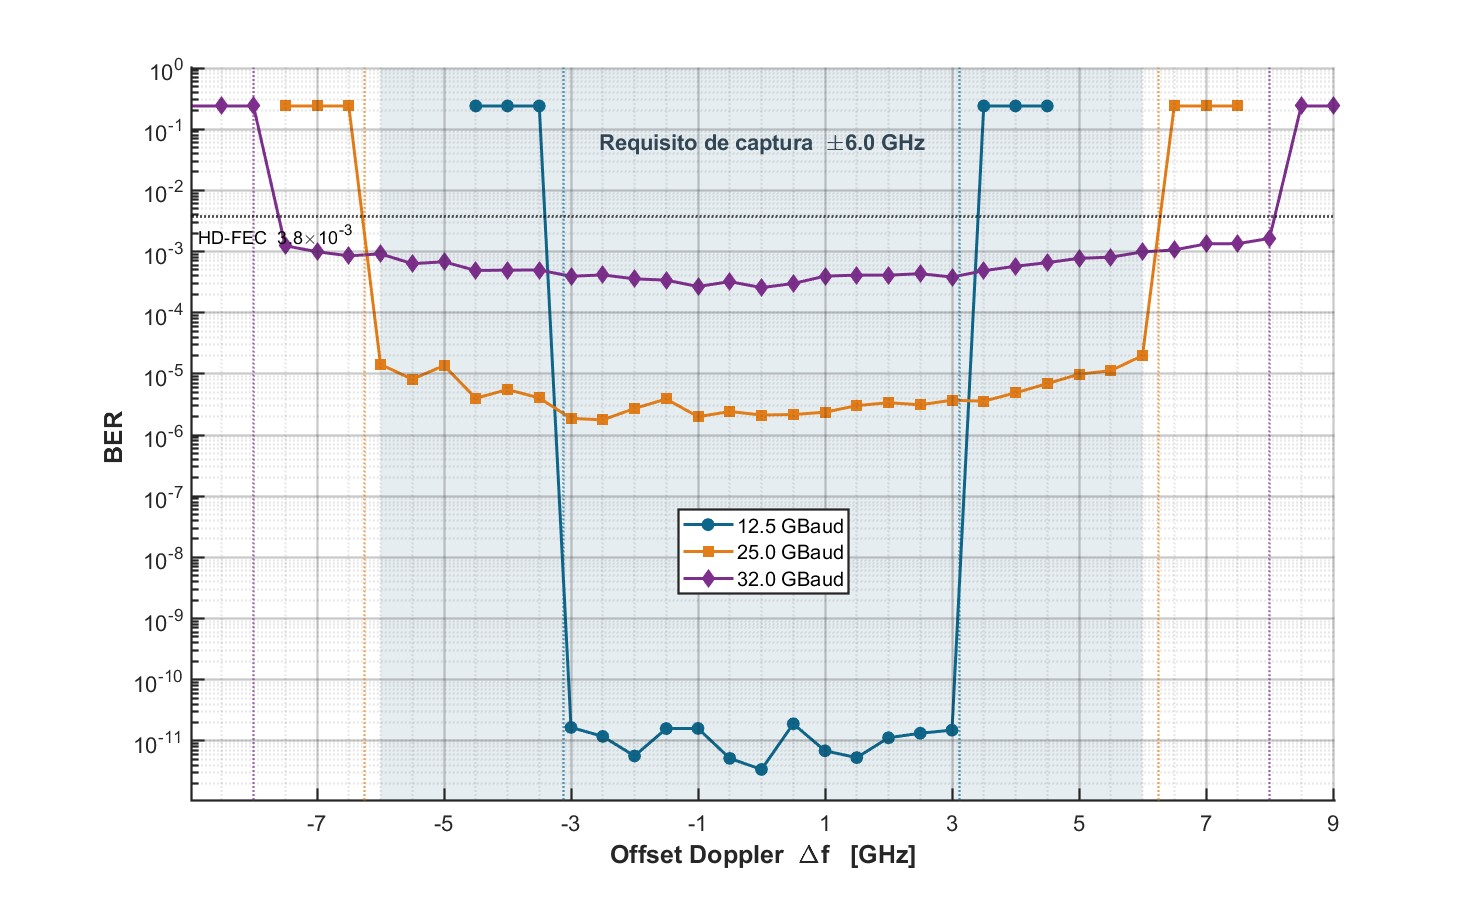
\includegraphics[width=0.92\textwidth]{figuras/DopplerComparacionExperimentalFinal.jpg}
  \caption[Barrido de offset Doppler medido en el laboratorio]{%
    BER estimada a partir del EVM contra offset de frecuencia medido en el
    laboratorio para las tres tasas, con tres pasadas por punto y paso de
    \SI{500}{\mega\hertz}. El piso de BER sube con la tasa por lo discutido en
    la \cref{sec:exp-osnr}.}
  \label{fig:exp-doppler}
\end{figure}

La \cref{fig:exp-doppler} muestra los resultados obtenidos. Las tres tasas
presentan un comportamiento similar. La BER estimada se mantiene
aproximadamente constante dentro del rango de funcionamiento del estimador de
frecuencia y aumenta abruptamente al superar su l\'imite de captura. En este
\'ultimo r\'egimen la estimaci\'on alcanza valores cercanos a \num{0.24},
correspondientes a un EVM de aproximadamente \SI{141}{\percent} al aplicar la
relaci\'on te\'orica utilizada para QPSK. Este incremento no representa
necesariamente una degradaci\'on progresiva de la calidad de la se\~nal, sino
que indica que el estimador de frecuencia deja de compensar correctamente el
offset, tal como se observ\'o en las simulaciones. Tambi\'en se aprecia un
ligero aumento de la BER dentro del rango de captura, a medida que crece el
valor absoluto del offset. Este comportamiento se analiza en la siguiente
secci\'on y se compara con los resultados de simulaci\'on.


\subsection{Espectro con y sin offset}
\label{sec:exp-doppler-espectro}

El efecto del offset sobre la se\~nal se ve directamente en el espectro de la
captura. La \cref{fig:exp-doppler-espectro-lab} compara dos medidas a
\SI{32}{\giga\baud}, una centrada y otra con un offset de
\SI{7}{\giga\hertz}.

\begin{figure}[H]
  \centering
  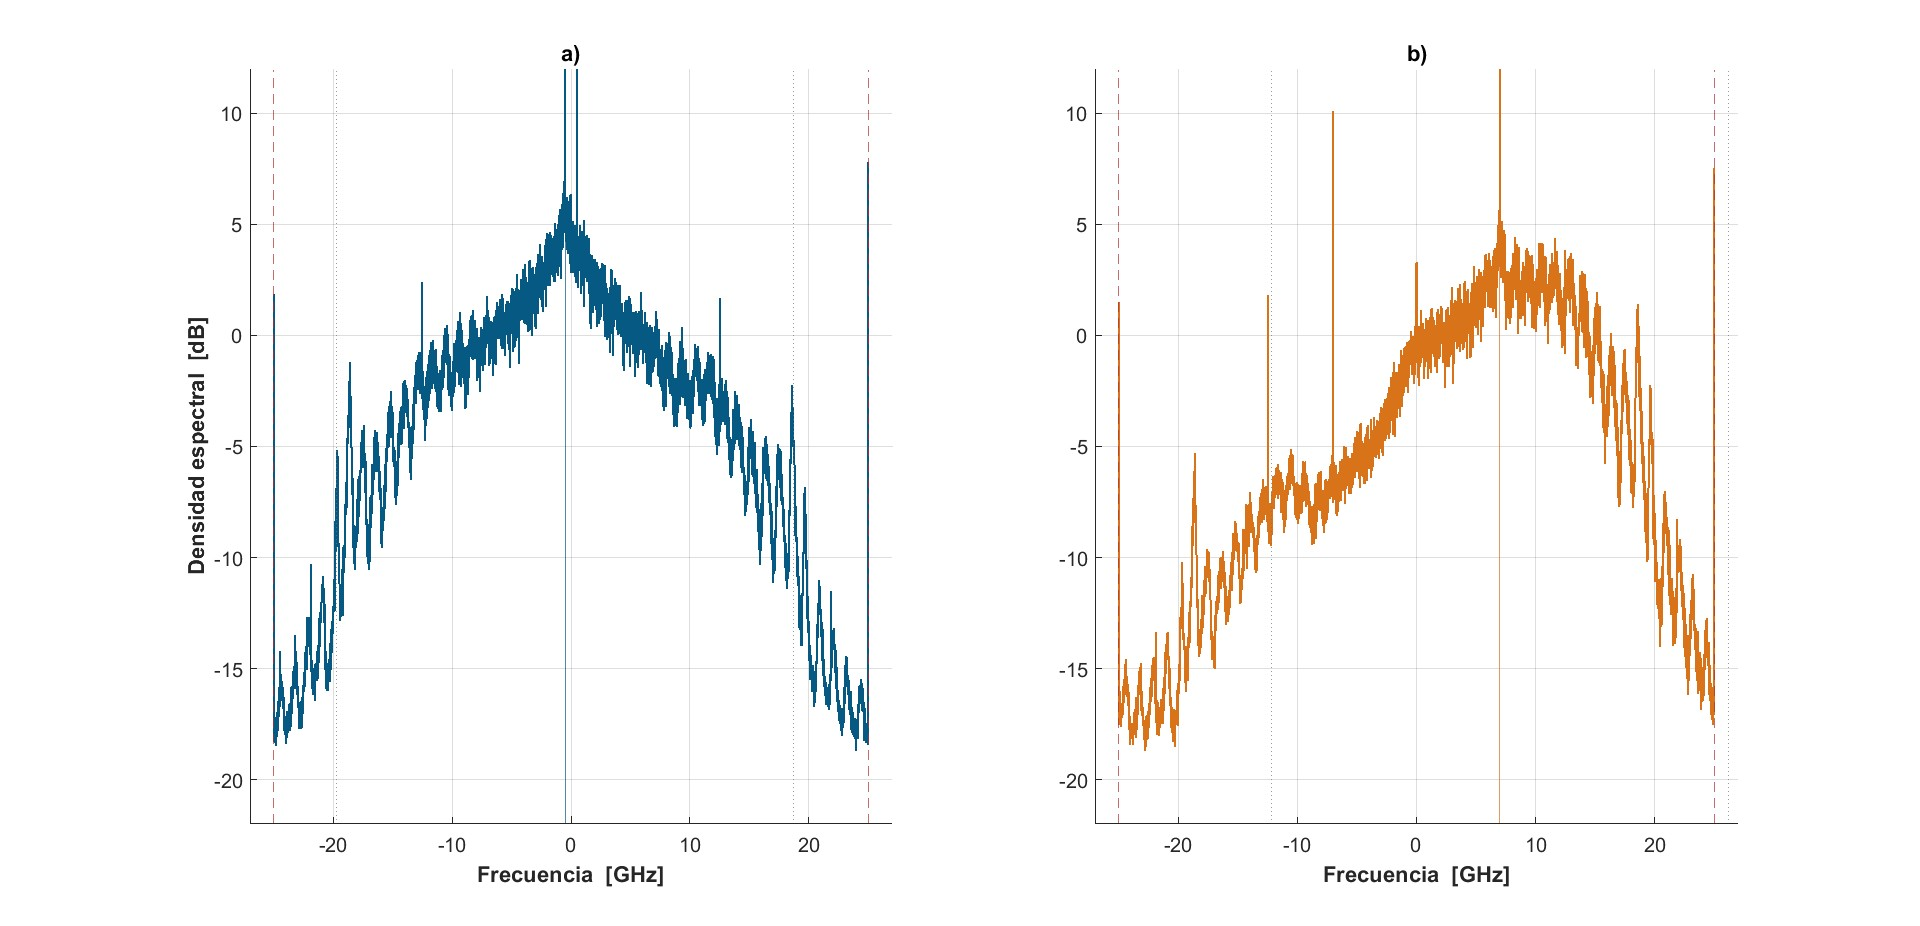
\includegraphics[width=\textwidth]{figuras/EspectroParaDistintosBW_LAB.jpg}
  \caption[Espectro medido con y sin offset Doppler]{%
    Densidad espectral de la se\~nal capturada a \SI{32}{\giga\baud}, a) sin
    offset y b) con un offset de \SI{7}{\giga\hertz}. Las l\'ineas de trazos
    marcan los \SI{\pm 25}{\giga\hertz} de Nyquist del osciloscopio.}
  \label{fig:exp-doppler-espectro-lab}
\end{figure}

Sin offset, el espectro de la se\~nal se encuentra centrado en continua y
presenta una distribuci\'on aproximadamente sim\'etrica respecto del origen.
Al introducir un offset, el espectro se desplaza en frecuencia. Debido a la
respuesta pasabajos del front end y del sistema de adquisici\'on, las
componentes desplazadas hacia frecuencias m\'as altas experimentan una mayor
atenuaci\'on, lo que introduce una distorsi\'on espectral asim\'etrica. A
\SI{32}{\giga\baud}, con un offset de \SI{7}{\giga\hertz}, parte del contenido
espectral de la se\~nal puede incluso superar el l\'imite de Nyquist del
osciloscopio, situado en \SI{25}{\giga\hertz}. Tambi\'en se observa el
desplazamiento de una componente residual de portadora, que permite
identificar visualmente el offset aplicado.

\begin{figure}[H]
  \centering
  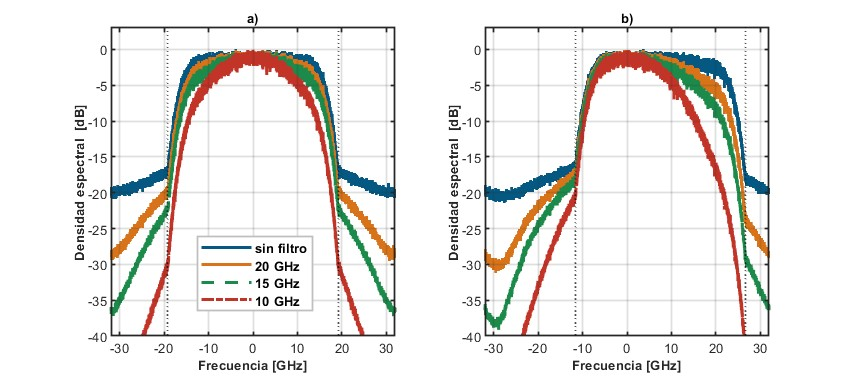
\includegraphics[width=\textwidth]{figuras/EspectroParaDistintosBWFotodiodos.jpg}
  \caption[Espectro simulado con y sin offset Doppler]{%
    Densidad espectral en simulaci\'on a \SI{32}{\giga\baud}, a) sin offset y
    b) con \SI{7}{\giga\hertz} de offset, para distintos anchos de banda. Las
    l\'ineas punteadas son los bordes de la banda de la se\~nal.}
  \label{fig:exp-doppler-espectro-sim}
\end{figure}

La \cref{fig:exp-doppler-espectro-sim} reproduce esta comparaci\'on mediante
simulaci\'on, considerando distintos anchos de banda para el filtro del
receptor. Mientras que la simulaci\'on utiliza pulsos conformados mediante un
filtro RRC, en el laboratorio se emplean se\~nales NRZ, por lo que sus
distribuciones espectrales son diferentes. Sin embargo, en ambos casos se
observa que el offset desplaza el espectro respecto de la respuesta en
frecuencia del receptor, produciendo una atenuaci\'on asim\'etrica que se
acent\'ua al reducir el ancho de banda. Este efecto contribuye a explicar el
aumento gradual de la BER observado dentro del rango de captura del estimador
de frecuencia, que se analiza con mayor detalle en la
\cref{sec:exp-comparacion}.




\section{Comparaci\'on con la simulaci\'on}
\label{sec:exp-comparacion}


\subsection{Constelaciones}

Las \cref{fig:exp-comp-125,fig:exp-comp-25,fig:exp-comp-32} son las
constelaciones que produce la simulaci\'on en las mismas tres tasas.

\begin{figure}[H]
  \centering
  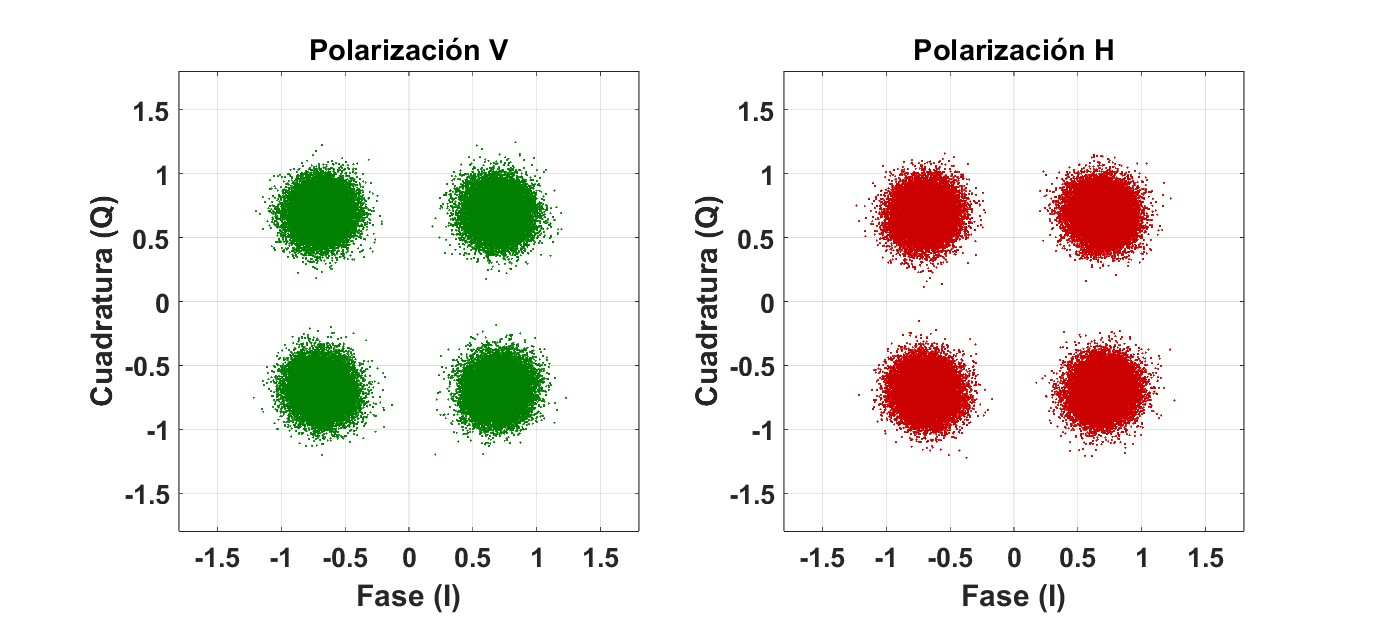
\includegraphics[width=0.95\textwidth]{figuras/Pol2_12p5Gb_Final.jpg}
  \caption[Constelaci\'on simulada a \SI{12.5}{\giga\baud}]{%
    Constelaci\'on de simulaci\'on a \SI{12.5}{\giga\baud}, para comparar con
    la \cref{fig:exp-const-125}.}
  \label{fig:exp-comp-125}
\end{figure}

\begin{figure}[H]
  \centering
  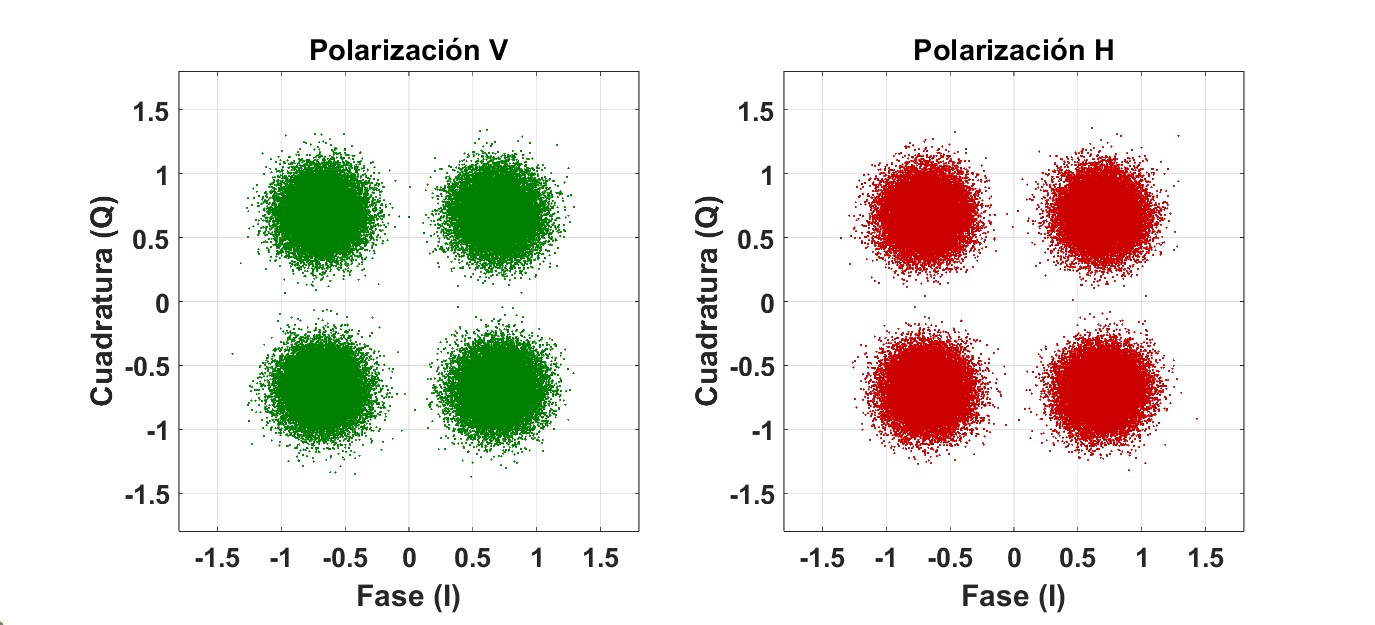
\includegraphics[width=0.95\textwidth]{figuras/Pol2_25Gb_Final.jpg}
  \caption[Constelaci\'on simulada a \SI{25}{\giga\baud}]{%
    Constelaci\'on de simulaci\'on a \SI{25}{\giga\baud}, para comparar con
    la \cref{fig:exp-const-25}.}
  \label{fig:exp-comp-25}
\end{figure}

\begin{figure}[H]
  \centering
  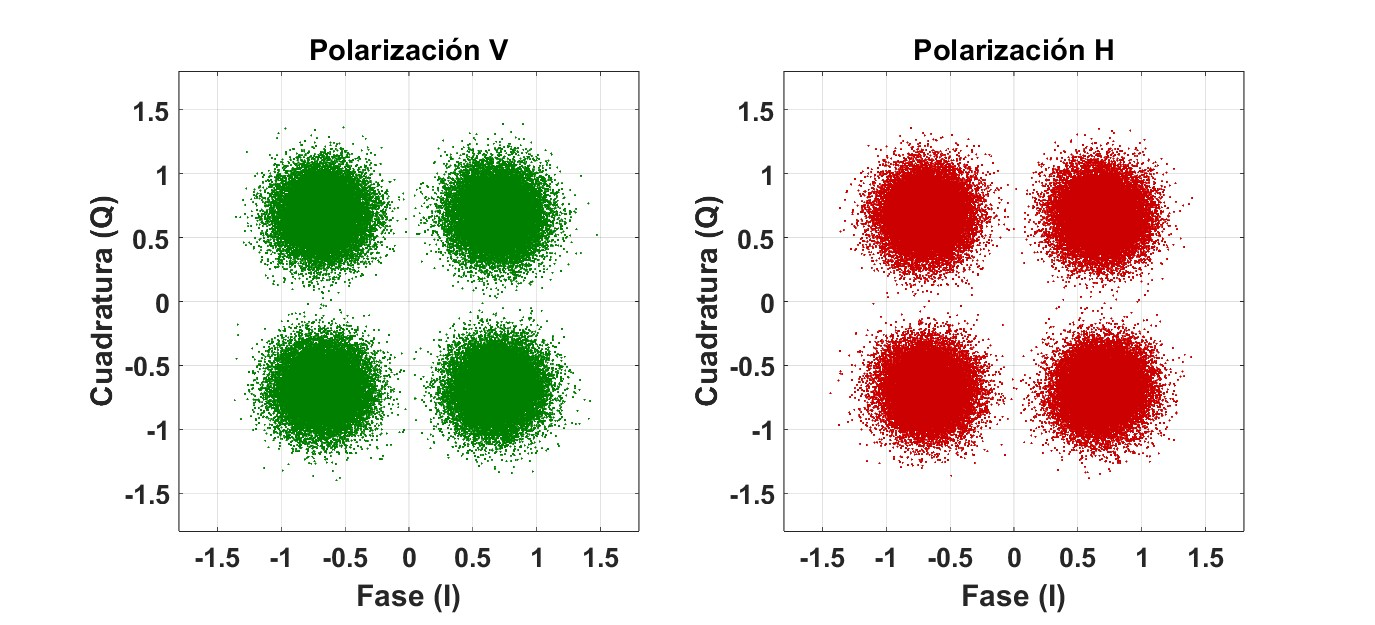
\includegraphics[width=0.95\textwidth]{figuras/Pol2_32Gb_Final.jpg}
  \caption[Constelaci\'on simulada a \SI{32}{\giga\baud}]{%
    Constelaci\'on de simulaci\'on a \SI{32}{\giga\baud}, para comparar con
    la \cref{fig:exp-const-32}.}
  \label{fig:exp-comp-32}
\end{figure}

La simulaci\'on se corri\'o al nivel de ruido que reproduce el EVM medido en cada
tasa, de modo que el tama\~no de las nubes no es una predicci\'on
independiente sino un ajuste. 
Compar\'andolas con las constelaciones obtenidas en el laboratorio, las
nubes simuladas son redondas y est\'an centradas en los mismos puntos, sin
rotaci\'on residual, sin elongaci\'on en una direcci\'on y sin sesgo entre las
dos polarizaciones. En cambio, las constelaciones finales del laboratorio parecen tener un 
desbalance de cuadratura que el GSOP no pudo compensar completamente.


\subsection{Tolerancia al offset Doppler}

Se reutiliza el gr\'afico del barrido de
offset simulado de la \cref{sec:tol-doppler} (\cref{fig:exp-doppler-sim}), con las mismas tres tasas que
la \cref{fig:exp-doppler}.

\begin{figure}[H]
  \centering
  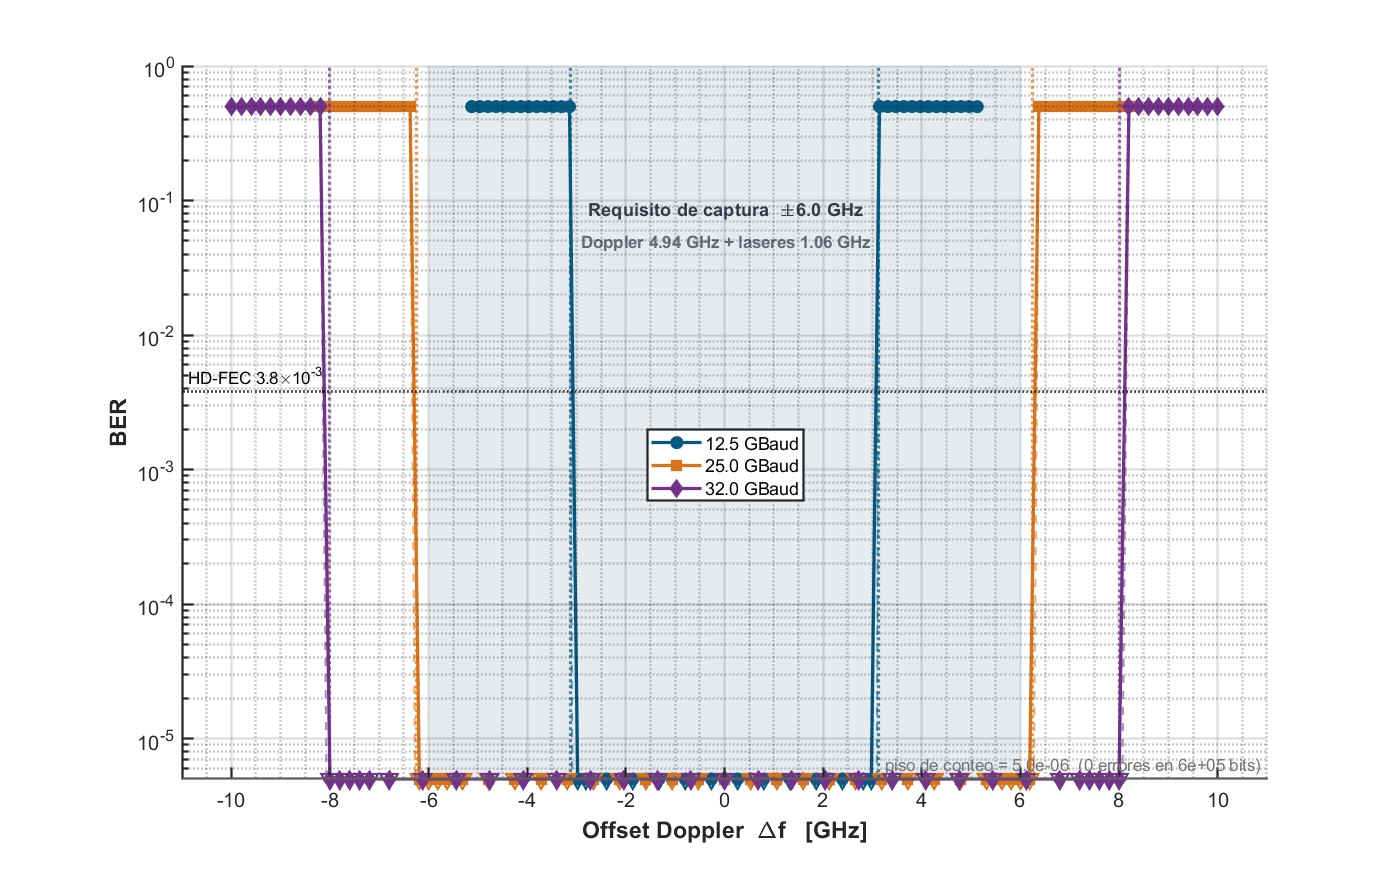
\includegraphics[width=0.92\textwidth]{figuras/EfectoDopplerFiguraFinalSimulacion.jpg}
  \caption[Barrido de offset Doppler en simulaci\'on]{%
    BER contra offset Doppler en simulaci\'on para las tres tasas de s\'imbolo,
    a OSNR fija. Es la misma figura de la \cref{fig:tol-doppler-sim},
    reproducida para comparar con la \cref{fig:exp-doppler}. La franja
    sombreada es el requisito de captura del enlace, \SI{\pm 6.0}{\giga\hertz},
    y la l\'inea de trazos el umbral HD-FEC.}
  \label{fig:exp-doppler-sim}
\end{figure}

La \cref{tab:exp-doppler} muestra el punto de corte medido contra el simulado
y contra el l\'imite te\'orico $\Rs/4$.

\begin{table}[htbp]
  \centering

  \begin{tabular}{lcccc}
    \toprule
    Tasa & $\Rs/4$ & Simulaci\'on & Laboratorio & Diferencia \\
    \midrule
    \SI{12.5}{\giga\baud} & \SI{3.125}{\giga\hertz} & \num{\pm 3.1}  & \num{\pm 3.0} & \SI{100}{\mega\hertz} \\
    \SI{25}{\giga\baud}   & \SI{6.25}{\giga\hertz}  & \num{\pm 6.25} & \num{\pm 6.0} & \SI{250}{\mega\hertz} \\
    \SI{32}{\giga\baud}   & \SI{8.0}{\giga\hertz}   & \num{\pm 8.0}  & $+8{,}0\,/\,-7{,}5$ & \SIrange{0}{500}{\mega\hertz} \\
    \bottomrule
  \end{tabular}
  \caption[Ventana de captura medida contra simulada]{%
    Offset de frecuencia donde el receptor falla, en laboratorio y en
    simulaci\'on, contra el l\'imite te\'orico $\Rs/4$.}
  \label{tab:exp-doppler}
\end{table}

Las tres tasas coinciden dentro de un paso de grilla, y fallan en
$\Rs/4$. En el laboratorio, el quiebre se presenta sistem\'aticamente un poco antes debido al paso de frecuencia entre mediciones. A su vez, existe un residuo de frecuencia entre los dos
l\'aseres de \SIrange{40}{95}{\mega\hertz} que puede correr
el punto de quiebre efectivo, lo que puede explicar la falla asim\'etrica en \SI{32}{\giga\baud}.



Dentro del rango enganchado hay una segunda diferencia. En el laboratorio
la BER aumenta ligeramente con el valor absoluto del offset, pero la simulaci\'on
no muestra esta pendiente. En el barrido contra la familia de OSNR de la
\cref{sec:tol-doppler-osnr}, a \SI{32}{\giga\baud} y \SI{16}{\dB}, el EVM
simulado pasa de \SI{26.57}{\percent} en \SI{0.2}{\giga\hertz} a
\SI{26.58}{\percent} en \SI{7.8}{\giga\hertz}, as\'i que la pendiente no
viene del procesamiento sino de los equipos. Adem\'as se observa que esta degradaci\'on crece con la tasa. A
\SI{12.5}{\giga\baud} casi no se aprecia, mientras que a \num{25} y
\SI{32}{\giga\baud}, la BER aumenta relativamente m\'as, lo que sugiere que el 
ancho de banda del receptor ocasiona el fen\'omeno. El offset desplaza el espectro de la se\~nal hacia uno de
los bordes de la banda del front-end y del osciloscopio, que est\'an
centradas en continua, y a \SI{32}{\giga\baud} el borde de la se\~nal llega a
los \SI{25}{\giga\hertz} de Nyquist del osciloscopio, que muestrea a
\SI{50}{\giga S\per\second}. En la simulaci\'on, en cambio, se utilizaron los anchos de banda
de las hojas de datos de los equipos, que resultaron ser m\'as grandes que los reales. En estas condiciones, y para 
los valores de Doppler que se manejan en el enlace,
el ancho de banda no es un limitante.


Para comprobarlo se repiti\'o el barrido de offset en simulaci\'on variando el
ancho de banda del receptor. La \cref{fig:exp-doppler-bw}
muestra el EVM resultante a la tasa de dise\~no.

\begin{figure}[H]
  \centering
  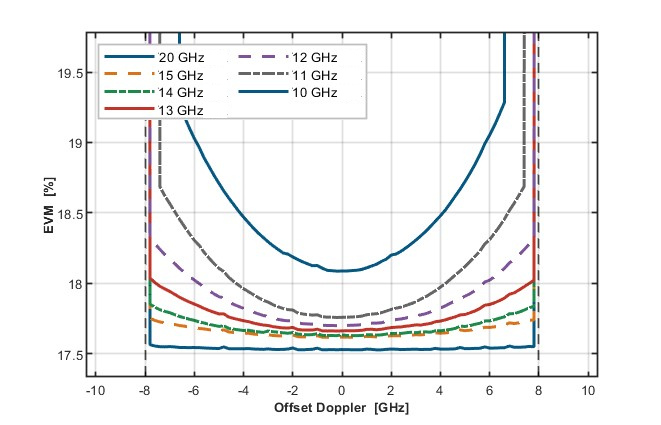
\includegraphics[width=0.8\textwidth]{figuras/BarridoOffsetDistintosBW.jpg}
  \caption[Barrido de offset Doppler para distintos anchos de banda]{%
    EVM contra offset Doppler en simulaci\'on a \SI{32}{\giga\baud}, para
    anchos de banda de receptor de \SIrange{10}{20}{\giga\hertz}. Las
    lineas verticales en $\pm\SI{8}{\giga\hertz}$ son el l\'imite de captura
    $\Rs/4$.}
  \label{fig:exp-doppler-bw}
\end{figure}

Con \SI{20}{\giga\hertz} de ancho de banda la curva es plana en todo el rango
enganchado, que es el caso de la \cref{fig:exp-doppler-sim}. Al achicar el
filtro el EVM sube en todo el barrido y, sobre todo, se curva. Con
\SI{10}{\giga\hertz} pasa de \SI{18.1}{\percent} en el centro a m\'as de
\SI{19}{\percent} en $\pm\SI{6.5}{\giga\hertz}$. Tambi\'en se observa que, por debajo de cierto valor
de ancho de banda, el rango \'util de captura disminuye, indicando que la señal qued\'o
filtrada por el receptor y el DSP no puede compensar la distorsi\'on.

El modelo reproduce entonces la pendiente medida en cuanto se le pone un ancho
de banda comparable al del laboratorio, lo que confirma que la
pendiente viene del equipo utilizado y no del procesamiento.


\section{Conclusiones}
\label{sec:exp-conclusiones}

El procesamiento recupera la constelaci\'on sobre se\~nales reales en las tres
tasas medidas, incluida la tasa de dise\~no de
\SI{128}{\giga\bit\per\second}, sin ninguna modificaci\'on respecto de la
versi\'on validada en simulaci\'on.

Los barridos de potencia dan la sensibilidad del conjunto. Sobre la BER
contada de la peor polarizaci\'on, el umbral HD-FEC se cruza con
\SI{-16.0}{\dBm} de se\~nal a \SI{12.5}{\giga\baud}, \SI{-13.6}{\dBm} a
\SI{25}{\giga\baud} y \SI{-11.0}{\dBm} a \SI{32}{\giga\baud}, los tres dentro
del rango de entrada que especifica el receptor. El primer escal\'on es del
orden de los \SI{3}{\dB} que cuesta duplicar la tasa de s\'imbolo y el segundo
vuelve a mostrar el exceso de la tasa de dise\~no que ya hab\'ia aparecido en
el punto de trabajo. Del lado del oscilador local el comportamiento es el de
un receptor coherente: por debajo de unos \SI{7}{\dBm} cada dec\'ibel se
traduce en un dec\'ibel de relaci\'on se\~nal-ruido, y por encima las curvas
se aplanan, de modo que llevar el oscilador al extremo alto de su rango no
agrega margen.


La tolerancia al offset Doppler medida en el laboratorio reproduce la simulada
en las tres tasas, confirmando el
l\'imite te\'orico de $\Rs/4$. Del lado del requisito, el resultado es el mismo
que en simulaci\'on. Utilizar una tasa de \SI{12.5}{\giga\baud} no cubre los
$\pm\SI{6.0}{\giga\hertz}$ del enlace, \SI{25}{\giga\baud} los cubre
justo, y \SI{32}{\giga\baud} los cubre con margen.

El ancho de banda el\'ectrico del camino de recepci\'on aparece como un segundo
efecto, separado del l\'imite de captura. Dentro del rango enganchado la BER
medida crece con el valor absoluto del offset, y la simulaci\'on reproduce esta
pendiente cuando se disminuye el ancho de banda del front end, de modo que viene del equipo
del laboratorio y no del procesamiento. Con los anchos de banda de las hojas de
datos la curva es plana, as\'i que para el rango de Doppler del enlace el
ancho de banda no es un limitante.


La limitaci\'on del laboratorio est\'a en el equipo utilizado, no en el receptor. La
frecuencia de muestreo del osciloscopio impide capturar la tasa de dise\~no
a dos muestras por s\'imbolo. 
Por \'ultimo, una comparaci\'on m\'as objetiva entre desempeños en el laboratorio 
y en la simulaci\'on ser\'ia posible midiendo OSNR directamente y no estim\'andola. Trazar la curva de BER contra OSNR, y compararla
contra la del cap\'itulo~\ref{cap:enlace}, es la continuaci\'on natural de
este trabajo.
